\PassOptionsToPackage{unicode}{hyperref}
\documentclass[aspectratio=1610, 11pt]{beamer}

\usepackage{amsmath}
\usepackage{amssymb}
\usetheme{tudo}

\title{Datenstrukturen, Algorithmen und Programmierung~2}
\author[A.~Coja-Oghlan]{Amin Coja-Oghlan}
\institute[DAP2]{Lehrstuhl Informatik 2\\Fakult\"at f\"ur Informatik}

\newcommand\dist{\mathrm{dist}}
\renewcommand{\vec}[1]{\boldsymbol{#1}}
\newcommand\NULL{{\tt NULL}}
\newcommand\dd{\mathrm d}
\newcommand\eul{\mathrm e}
\newcommand\cA{\mathcal A}
\newcommand\cB{\mathcal B}
\newcommand\cC{\mathcal C}
\newcommand\cD{\mathcal D}
\newcommand\cE{\mathcal E}
\newcommand\cF{\mathcal F}
\newcommand\cG{\mathcal G}
\newcommand\cH{\mathcal H}
\newcommand\cI{\mathcal I}
\newcommand\cJ{\mathcal J}
\newcommand\cK{\mathcal K}
\newcommand\cL{\mathcal L}
\newcommand\cM{\mathcal M}
\newcommand\cN{\mathcal N}
\newcommand\cO{\mathcal O}
\newcommand\cP{\mathcal P}
\newcommand\cQ{\mathcal Q}
\newcommand\cR{\mathcal R}
\newcommand\cS{\mathcal S}
\newcommand\cT{\mathcal T}
\newcommand\cU{\mathcal U}
\newcommand\cV{\mathcal V}
\newcommand\cW{\mathcal W}
\newcommand\cX{\mathcal X}
\newcommand\cY{\mathcal Y}
\newcommand\cZ{\mathcal Z}
\newcommand\fA{\mathfrak A}
\newcommand\fB{\mathfrak B}
\newcommand\fC{\mathfrak C}
\newcommand\fD{\mathfrak D}
\newcommand\fE{\mathfrak E}
\newcommand\fF{\mathfrak F}
\newcommand\fG{\mathfrak G}
\newcommand\fH{\mathfrak H}
\newcommand\fI{\mathfrak I}
\newcommand\fJ{\mathfrak J}
\newcommand\fK{\mathfrak K}
\newcommand\fL{\mathfrak L}
\newcommand\fM{\mathfrak M}
\newcommand\fN{\mathfrak N}
\newcommand\fO{\mathfrak O}
\newcommand\fP{\mathfrak P}
\newcommand\fQ{\mathfrak Q}
\newcommand\fR{\mathfrak R}
\newcommand\fS{\mathfrak S}
\newcommand\fT{\mathfrak T}
\newcommand\fU{\mathfrak U}
\newcommand\fV{\mathfrak V}
\newcommand\fW{\mathfrak W}
\newcommand\fX{\mathfrak X}
\newcommand\fY{\mathfrak Y}
\newcommand\fZ{\mathfrak Z}
\newcommand\fa{\mathfrak a}
\newcommand\fb{\mathfrak b}
\newcommand\fc{\mathfrak c}
\newcommand\fd{\mathfrak d}
\newcommand\fe{\mathfrak e}
\newcommand\ff{\mathfrak f}
\newcommand\fg{\mathfrak g}
\newcommand\fh{\mathfrak h}
%\newcommand\fi{\mathfrak i}
\newcommand\fj{\mathfrak j}
\newcommand\fk{\mathfrak k}
\newcommand\fl{\mathfrak l}
\newcommand\fm{\mathfrak m}
\newcommand\fn{\mathfrak n}
\newcommand\fo{\mathfrak o}
\newcommand\fp{\mathfrak p}
\newcommand\fq{\mathfrak q}
\newcommand\fr{\mathfrak r}
\newcommand\fs{\mathfrak s}
\newcommand\ft{\mathfrak t}
\newcommand\fu{\mathfrak u}
\newcommand\fv{\mathfrak v}
\newcommand\fw{\mathfrak w}
\newcommand\fx{\mathfrak x}
\newcommand\fy{\mathfrak y}
\newcommand\fz{\mathfrak z}
\newcommand\vA{\vec A}
\newcommand\vB{\vec B}
\newcommand\vC{\vec C}
\newcommand\vD{\vec D}
\newcommand\vE{\vec E}
\newcommand\vF{\vec F}
\newcommand\vG{\vec G}
\newcommand\vH{\vec H}
\newcommand\vI{\vec I}
\newcommand\vJ{\vec J}
\newcommand\vK{\vec K}
\newcommand\vL{\vec L}
\newcommand\vM{\vec M}
\newcommand\vN{\vec N}
\newcommand\vO{\vec O}
\newcommand\vP{\vec P}
\newcommand\vQ{\vec Q}
\newcommand\vR{\vec R}
\newcommand\vS{\vec S}
\newcommand\vT{\vec T}
\newcommand\vU{\vec U}
\newcommand\vV{\vec V}
\newcommand\vW{\vec W}
\newcommand\vX{\vec X}
\newcommand\vY{\vec Y}
\newcommand\vZ{\vec Z}
\newcommand\va{\vec a}
\newcommand\vb{\vec b}
\newcommand\vc{\vec c}
\newcommand\vd{\vec d}
\newcommand\ve{\vec e}
\newcommand\vf{\vec f}
\newcommand\vg{\vec g}
\newcommand\vh{\vec h}
\newcommand\vi{\vec i}
\newcommand\vj{\vec j}
\newcommand\vk{\vec k}
\newcommand\vl{\vec l}
\newcommand\vm{\vec m}
\newcommand\vn{\vec n}
\newcommand\vo{\vec o}
\newcommand\vp{\vec p}
\newcommand\vq{\vec q}
\newcommand\vr{\vec r}
\newcommand\vs{\vec s}
\newcommand\vt{\vec t}
\newcommand\vu{\vec u}
\renewcommand\vv{\vec v}
\newcommand\vw{\vec w}
\newcommand\vx{\vec x}
\newcommand\vy{\vec y}
\newcommand\vz{\vec z}
\renewcommand\AA{\mathbb A}
\newcommand\NN{\mathbb N}
\newcommand\ZZ{\mathbb Z}
\newcommand\PP{\mathbb P}
\newcommand\QQ{\mathbb Q}
\newcommand\RR{\mathbb R}
\newcommand\RRpos{\mathbb R_{\geq0}}
\newcommand\QQpos{\mathbb Q_{\geq0}}
\renewcommand\SS{\mathbb S}
\newcommand\CC{\mathbb C}
\newcommand{\ord}{\mathrm{ord}}
\newcommand{\id}{\mathrm{id}}
\newcommand{\pr}{\mathrm{P}}
\newcommand{\Vol}{\mathrm{vol}}
\newcommand\norm[1]{\left\|{#1}\right\|} 
\newcommand\sign{\mathrm{sign}}
\newcommand{\eps}{\varepsilon}
\newcommand{\abs}[1]{\left|#1\right|}
\newcommand\bc[1]{\left({#1}\right)} 
\newcommand\cbc[1]{\left\{{#1}\right\}} 
\newcommand\bcfr[2]{\bc{\frac{#1}{#2}}} 
\newcommand{\bck}[1]{\left\langle{#1}\right\rangle} 
\newcommand\brk[1]{\left\lbrack{#1}\right\rbrack} 
\newcommand\scal[2]{\bck{{#1},{#2}}} 
\newcommand{\vecone}{\mathbb{1}}
\newcommand{\tensor}{\otimes}
\newcommand{\diag}{\mathrm{diag}}
\newcommand{\ggt}{\mathrm{ggT}}
\newcommand{\kgv}{\mathrm{kgV}}
\newcommand{\trans}{\top}
\newcommand{\Karonski}{Karo\'nski}
\newcommand{\Erdos}{Erd\H{o}s}
\newcommand{\Renyi}{R\'enyi}
\newcommand{\Lovasz}{Lov\'asz}
\newcommand{\Juhasz}{Juh\'asz}
\newcommand{\Bollobas}{Bollob\'as}
\newcommand{\Furedi}{F\"uredi}
\newcommand{\Komlos}{Koml\'os}
\newcommand{\Luczak}{\L uczak}
\newcommand{\Kucera}{Ku\v{c}era}
\newcommand{\Szemeredi}{Szemer\'edi}

\newcommand{\mytitle}{Amortisierte Analyse}

\begin{document}

\frame[plain]{\titlepage}

\begin{frame}\frametitle{\mytitle}
	\begin{exampleblock}{Worum geht es?}
		\begin{itemize}
			\item Datenstrukturen sind wichtige Hilfsmittel der Algorithmik
			\item \alert{Beispiele:} Stacks, Splay Trees, Fibonacci Heaps\dots
			\item Die meisten Operationen ben\"otigen wenig Zeit
			\item Ab und zu ist aber ``Aufr\"aumen'' n\"otig
			\item \emph{Idee:} Analyse der Gesamtlaufzeit durch kreative Buchf\"uhrung 
		\end{itemize}
	\end{exampleblock}
\end{frame}


\begin{frame}\frametitle{Beispiel: Stapel}
	\begin{exampleblock}{Datenstruktur Stapel}
		\begin{itemize}
			\item Funktionalit\"at: {\tt push}, {\tt pop}, {\tt empty}
			\item Abzubilden im Hauptspeicher (`random access')
			\item Zahl der zu speichernden Eintr\"age a priori unbekannt
			\item \emph{Ziel:} Zeit-- und Speicherplatzeffizienz.
		\end{itemize}
	\end{exampleblock}
\end{frame}

\begin{frame}\frametitle{Beispiel: Stapel}
	\begin{overprint} 
		\onslide<1>\hspace{50mm}
\includegraphics[height=4mm]{images/stack00.pdf}
		\onslide<2>\hspace{50mm}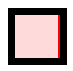
\includegraphics[height=4mm]{images/stack01.pdf}
		\onslide<3>\hspace{50mm}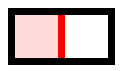
\includegraphics[height=4mm]{images/stack02.pdf}
		\onslide<4>\hspace{50mm}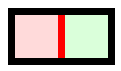
\includegraphics[height=4mm]{images/stack03.pdf}
		\onslide<5>\hspace{50mm}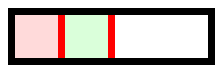
\includegraphics[height=4mm]{images/stack04.pdf}
		\onslide<6>\hspace{50mm}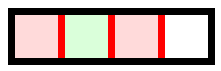
\includegraphics[height=4mm]{images/stack05.pdf}
		\onslide<7>\hspace{50mm}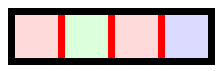
\includegraphics[height=4mm]{images/stack06.pdf}
		\onslide<8>\hspace{50mm}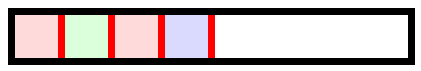
\includegraphics[height=4mm]{images/stack07.pdf}
		\onslide<9>\hspace{50mm}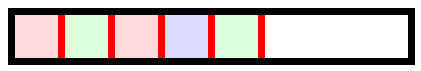
\includegraphics[height=4mm]{images/stack08.pdf}
	\end{overprint}
	\begin{exampleblock}{Umsetzung}
		\begin{itemize}
			\item Reserviere einen Speicherblock der Gr\"o\ss e $n$
			\item Anfangs $n=1$
			\item Wenn der Block voll ist, reserviere einen Block der Gr\"o\ss e $2n$
			\item Kopiere den Inhalt des alten Blocks in den neuen
			\item $\leadsto$ einzelne {\tt push}-Operation zeitintensiv
			\item (Freigeben von Speicherplatz normalerweise einfacher.)
		\end{itemize}
	\end{exampleblock}
\end{frame}

\begin{frame}\frametitle{Beispiel: Stapel}
	\begin{exampleblock}{Beispiel: $N\times${\tt push}, $N\times${\tt pop}}
		\begin{itemize}
			\item Nehmen wir an, $N=2^k$ ist eine Potenz von $2$.
			\item Dann wird bei den {\tt push}-Operationen
				\begin{align*}
					2,\quad3,\quad5,\quad9,\quad17,\quad\ldots,\quad2^{k-1}+1
				\end{align*}
				jeweils die Gr\"o\ss e des Speicherblocks verdoppelt.
			\item Der Zeitbedarf f\"ur die letzte Verdopplung allein ist
				\begin{align*}
					2^{k-1}+1>N/2.
				\end{align*}
			\item \emph{Naive Analyse:} Zeitbedarf $O(N^2)$
		\end{itemize}
	\end{exampleblock}
\end{frame}

\begin{frame}\frametitle{Beispiel: Stapel}
	\begin{exampleblock}{Amortisierte Analyse}
		\begin{itemize}
			\item Angenommen insgesamt $N$ {\tt push}-Operationen
			\item \emph{Behauptung:} Gesamtlaufzeit $O(N)$
		\end{itemize}
	\end{exampleblock}
\end{frame}

\begin{frame}\frametitle{Beispiel: Stapel}
	\begin{exampleblock}{Amortisierte Analyse}
		\begin{itemize}
			\item Angenommen insgesamt $N$ {\tt push}-Operationen
			\item \emph{Behauptung:} Gesamtlaufzeit $O(N)$
			\item \alert{Direkte Analyse:} Zeitaufwand f\"ur Reallokation.
			\item Mit $\ell=\lceil\log_2N\rceil$ ist dieser beschr\"ankt durch
				\begin{align*}
					\sum_{i=1}^{\ell}2^{i-1}=\sum_{i=0}^{\ell-1}2^i\leq2^\ell=O(N).
				\end{align*}
		\end{itemize}
	\end{exampleblock}
\end{frame}

\begin{frame}\frametitle{Beispiel: Stapel}
	\begin{exampleblock}{Amortisierte Analyse}
		\begin{itemize}
			\item Angenommen insgesamt $N$ {\tt push}-Operationen
			\item Gesamtlaufzeit $O(N)$
			\item Die \emph{amortisierte Laufzeit} pro {\tt push} ist also $O(1)$
		\end{itemize}
	\end{exampleblock}
\end{frame}

\begin{frame}\frametitle{Amortisierte Analyse}
	\begin{exampleblock}{Informelle Definition}
		\begin{itemize}
			\item Angenommen die tats\"achlichen Kosten einer Folge von Operationen sind
				\begin{align*}
					c_1,c_2,\ldots,c_N\geq0
				\end{align*}
			\item Sei $c_1',\ldots,c_N'$ eine weitere Folge, so da\ss
				\begin{align*}
					c_1+c_2+\cdots+c_i&\leq c_1'+c_2'+\cdots+c_i'&&\mbox{f\"ur alle }1\leq i\leq N.
				\end{align*}
			\item Dann ist $c_1',\ldots,c_N'$ eine \emph{Amortisierung} von $c_1,\ldots,c_N$.
			\item Die \emph{amortisierten Gesamtkosten} sind $c_1'+\cdots+c_N'$.
		\end{itemize}
	\end{exampleblock}
\end{frame}

\begin{frame}\frametitle{Amortisierte Analyse}
	\hfill
	{\begin{tabular}{c|c|c}
			Woche&Kosten&Amortisierung\\\hline
			1&$c_1=0$&$c_1'=10$\\
			2&$c_2=0$&$c_2'=10$\\
			3&$c_3=0$&$c_3'=10$\\
			4&$c_4=0$&$c_4'=10$\\
			5&$c_5=50$&$c_5'=10$
	\end{tabular}}
	\begin{exampleblock}{Beispiel Fahrrad}
		\begin{itemize}
			\item Angenommen ich radle t\"aglich zur Uni
			\item Die meisten Tage entstehen keine Kosten 
			\item Aber gelegentlich entstehen (relativ) hohe Reparaturkosten
			\item \emph{Idee:} lege diese Kosten auf alle Tage/Kilometer um\dots
			\item \dots um die Gesamtkosten einfacher kalkulieren zu k\"onnen 
		\end{itemize}
	\end{exampleblock}
\end{frame}

\begin{frame}\frametitle{Amortisierte Analyse}
	\begin{exampleblock}{Potentialfunktionen}
		\begin{itemize}
			\item Wie findet man eine geeignete Amortisierung?
			\item \alert{Hilfsmittel:} Potentialfunktion $\Phi:\mathcal Z\to\mathbb R_{\geq0}$
			\item \emph{Idee:} $\Phi$ misst die 'Unordnung' des aktuellen Zustands
			\item F\"ur eine leere Datenstruktur gelte $\Phi(\emptyset)=0$
			\item Wenn $z_0=\emptyset,z_1,\ldots,z_N$ die Zust\"ande der Datenstruktur sind, definiere
				\begin{align*}
					c_i'&=c_i+\Phi(z_i)-\Phi(z_{i-1})
				\end{align*}
		\end{itemize}
	\end{exampleblock}
\end{frame}

\begin{frame}\frametitle{Amortisierte Analyse}
	\begin{exampleblock}{Potentialfunktionen}
		\begin{itemize}
			\item Wir definieren 
				\begin{align*}
					c_i'&=c_i+\Phi(z_i)-\Phi(z_{i-1})&&(i\geq1)
				\end{align*}
			\item \emph{Behauptung:} $c_1+\cdots+c_i\leq c_1'+\cdots+c_i'$ f\"ur alle $i$
			\item Zum Beweis berechnen wir
				\begin{align*}
					c_1'+\cdots+c_i'&=(c_1+\Phi(z_1)-\Phi(z_0))+\cdots+(c_i+\Phi(z_i)-\Phi(z_{i-1}))\\
									&=c_1+\cdots+c_i+(\Phi(z_1)-\Phi(z_0))+\cdots+(\Phi(z_i)-\Phi(z_{i-1}))\\
									&=c_1+\cdots+c_i+\Phi(z_i)-\Phi(z_0)\\
									&=c_1+\cdots+c_i+\Phi(z_i)\geq c_1+\cdots+c_i
				\end{align*}
		\end{itemize}
	\end{exampleblock}
\end{frame}

\begin{frame}\frametitle{Beispiel Stapel}
	\begin{exampleblock}{Analyse via Potentialfunktion}
		\begin{itemize}
			\item Der Zustand $z_i$ besteht aus
				\begin{align*}
					b_i&=\#\mbox{belegte Pl\"atze},&n_i&=\mbox{reservierter Speicherplatz}
				\end{align*}
			\item Wir definieren
				\begin{align*}
					\Phi(z_i)=\max\{0,2b_i-n_i\}
				\end{align*}
		\end{itemize}
	\end{exampleblock}
\end{frame}

\begin{frame}\frametitle{Beispiel Stapel}
	\begin{exampleblock}{Analyse via Potentialfunktion}
		\begin{itemize}
			\item Die Potentialfunktion ist $\Phi(z_i)=\max\{0,2b_i-n_i\}$
			\item Amortisierte Kosten:
				\begin{align*}
					c_i'&=3&&\mbox{f\"ur {\tt push} ohne Vergr\"o\ss ern}\\
					c_i'&=3&&\mbox{f\"ur {\tt push} mit Vergr\"o\ss ern}\\
					c_i'&=-1&&\mbox{f\"ur {\tt pop}}
				\end{align*}
			\item Also $c_i'=O(1)$ f\"ur alle $i$
			\item Folglich $c_1+\cdots+c_N=O(N)$
		\end{itemize}
	\end{exampleblock}
\end{frame}

\begin{frame}\frametitle{Weitere Beispiele}
	\begin{itemize}
		\item \alert{Splay trees:} amortisiert $O(\log n)$ {\tt search}, {\tt insert}, {\tt delete}
		\item \alert{Dictionary:} amortisiert $O(\log n)$ {\tt insert}
		\item \alert{Fibonacci heap:} amortisiert $O(1)$ {\tt insert}, {\tt findMin}, {\tt decKey}; $O(\log n)$ {\tt delMin}
	\end{itemize}
\end{frame}

\begin{frame}\frametitle{Anwendung: Dijkstra-Algorithmus}
	\hfill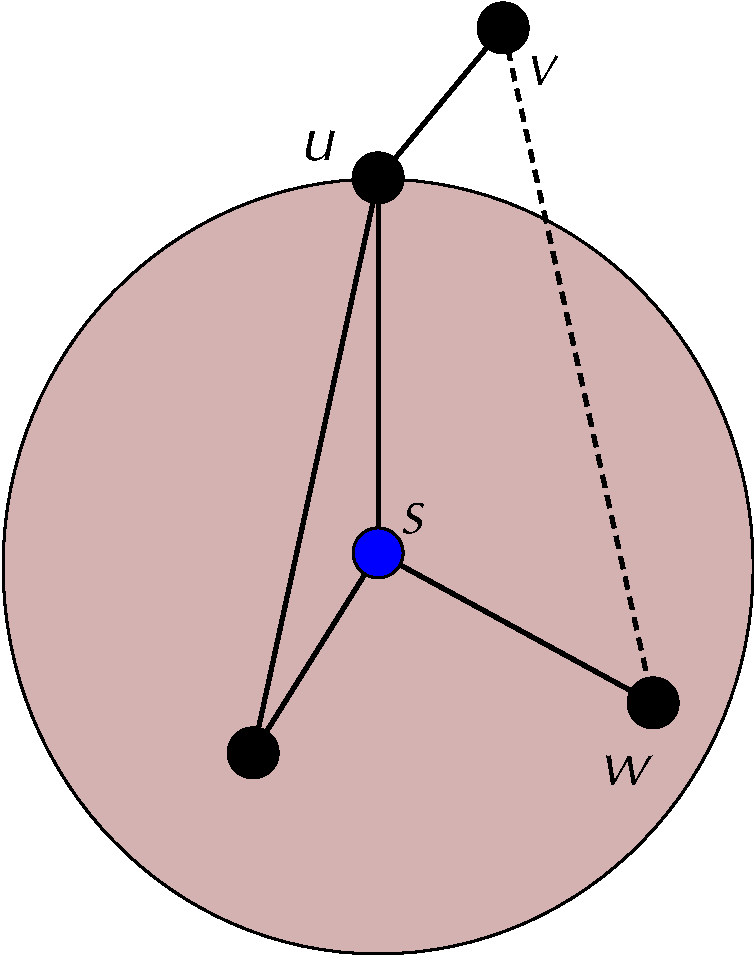
\includegraphics[height=25mm]{images/DijkstraIllustr.pdf}
	\begin{exampleblock}{Dijkstra-Algorithmus}
		%\alert{Eingabe:} Graph $G$ mit Kantenl\"angen $\ell(e)\geq0$; Knoten $s,t$\\
		%\alert{Ausgabe:} Abstand von $s,t$
		\begin{enumerate}
			\item Setze anfangs $d(s)=0$, $d(v)=\infty$ f\"ur alle $v\in V\setminus\{s\}$
			\item F\"uge alle $v\in V$ in eine Fibonaccihalde mit Schl\"ussel $d(v)$
			\item Solange die Halde nicht leer ist
			\item $\quad$ entnehme minimales Element $u$
			\item $\quad$ reduziere $d(v)\leftarrow \min\{d(v),d(u)+\ell(u,v)\}$ f\"ur alle $v\in\partial u$
			\item Gib $d(t)$ aus
		\end{enumerate}
	\end{exampleblock}
\end{frame}

\begin{frame}\frametitle{Anwendung: Dijkstra-Algorithms}
	\begin{block}{Satz}
		Der Dijkstra-Algorithmus hat Laufzeit $O(|E_G|+|V_G|\log|V_G|)$. 
	\end{block}
	\begin{overprint}
		\onslide<1>
		\begin{exampleblock}{Beweis}
			\begin{itemize}
				\item Jeder Knoten wird nur einmal der Halde hinzugef\"ugt/entfernt
				\item Gesamtaufwand daf\"ur ist $O(|V_G|\log|V_G|)$
				\item Ferner wird f\"ur jede Kante einmal {\tt decKey} aufgerufen
				\item Laufzeit daf\"ur $O(|E|)$
			\end{itemize}
		\end{exampleblock}
	\end{overprint}
\end{frame}

\begin{frame}\frametitle{Zusammenfassung}
	\begin{exampleblock}{}
		\begin{itemize}
			\item Amortisierung ist ein Analysewerkzeug f\"ur Datenstrukturen 
			\item \alert{Ziel:} Gesamtlaufzeit \"uber viele Operationen bestimmen
			\item \alert{Hilfsmittel:} Potentialfunktionen
			\item \alert{Einschr\"ankungen:} z.B.\ kritische Reaktionszeiten
		\end{itemize}
	\end{exampleblock}
\end{frame}

\end{document}
